\documentclass[12pt]{article}

\usepackage[english]{babel}
\usepackage[utf8]{inputenc}
\usepackage{sansmathfonts}
\usepackage[T1]{fontenc}
\renewcommand*\familydefault{\sfdefault} %% Only if the base font of the document is to be sans serif
\usepackage{multicol,lipsum}
\usepackage{amsmath,cancel}
\usepackage{amssymb,amsthm,dsfont,mathrsfs}
\usepackage[colorinlistoftodos]{todonotes}
\usepackage{geometry}
\geometry{
a4paper,
total={170mm,257mm},
left=20mm,
top=15mm,
bottom=22mm,
}
\usepackage{natbib}
\usepackage{soul}
\usepackage{setspace}
\usepackage{hyperref}
\usepackage{xcolor}
\usepackage{graphicx}
\usepackage{tikz}
\usepackage{siunitx}
\graphicspath{ {imagens/} }
\usepackage{fancyhdr}
\pagestyle{fancy}
\renewcommand{\headrulewidth}{0pt}

\color{darkgray}
\newcommand{\T}[1]{\vspace{0.4cm}\textbf{\large#1}}
\newcommand{\TW}[1]{\textbf{\large#1}}

\newcommand{\TM}[1]{\vspace{0.2cm} \textbf{#1}}

\newcommand{\M}[1]{
\vspace{-0.6cm}
\begin{flalign*}
#1&
\end{flalign*}
\vspace{-0.6cm}
}


\definecolor{bluebell}{rgb}{0.25, 0.35, 0.89} 
\definecolor{laranja}{rgb}{0.87, 0.48, 0.25} 
\definecolor{verde}{rgb}{0, 0.54, 0.44} 
\definecolor{babypink}{rgb}{1, 0.42, 0.52} 
\definecolor{rosa}{rgb}{1, 0.72, 0.77} 
\definecolor{cinza}{rgb}{0.3, 0.3, 0.3}  
\definecolor{iris}{rgb}{0.25, 0.35, 0.89}  
\definecolor{babyblue}{rgb}{0.13, 0.59, 0.95}

\setlength\columnsep{30pt}

\setlength{\parindent}{0cm}
\setlength{\fboxrule}{1.3pt}  % <-- Aumenta a espessura

\newcommand{\Formula}[1]{
\begin{center}
\color{iris}
\fcolorbox{rosa}{white}{
\(
\begin{array}{c}
#1
\end{array}
\)
}
\color{cinza}
\end{center}
}

\begin{document}
\pagenumbering{gobble}
\setstretch{1.3}


\includegraphics[width=4cm]{Logo2.png}
\begin{center}
    \textbf{\Huge \textcolor{bluebell}{Função Afim}}
\end{center}

\begin{multicols}{2}

\TW{Função Afim} 

A função afim é também conhecida como função de 1º grau e é uma função $f : \mathbb{R} \rightarrow \mathbb{R}$ definida como $f(x) = ax +b$, onde $a, b \in \mathbb{R}$. Nessa função o valor de $a$ representa o coeficiente angular da reta, ou seja, é a taxa de variação da função. O valor de $b$ representa o coeficiente linear da reta, ou seja, é o valor da função quando $x=0$. Essa função no plano cartesiano é representada por $y=ax+b$.

\TM{Exemplos:}

$f(x) = 3x+4$
\vspace{0.3cm}

Temos que o coeficiente angular é igual a $3$ e o coeficiente linear é igual a $4$.

Para calcular o valor de $f(2)$ temos:

$f(2) = 3 \cdot 2 + 4$

$f(2) = 6+4$

$f(2) = 10$

\TM{Coeficiente Angular}

Para calcular o coeficiente angular dado dois pontos $A=(x_A,y_A)$ e $B=(x_B,y_B)$ basta calcular a distância a variação dos dois pontos no eixo $y$ dividido pela variação em $x$.

\Formula{
a=\dfrac{\Delta y}{\Delta x} = \dfrac{y_B - y_A}{x_B-x_A}
}

\TM{Exemplos:}

Dados os pontos $A=(2,3)$ e $B=(3,5)$, temos que:

\vspace{8px}
$a=\dfrac{5-3}{3-2}$ \vspace{8px}

$a=\dfrac{2}{1}$ \vspace{8px}

$a=2$

\TM{Coeficiente Linear}

Para calcular o coeficiente linear dado dois pontos $A$ e $B$ é necessário calcular o coeficiente angular $a$ e em seguida calcular o valor de $b$ utilizando um ponto pertencente à reta.

\TM{Exemplos:}

Dado o seguinte gráfico, podemos calcular o coeficiente linear da seguinte forma:

\begin{center}
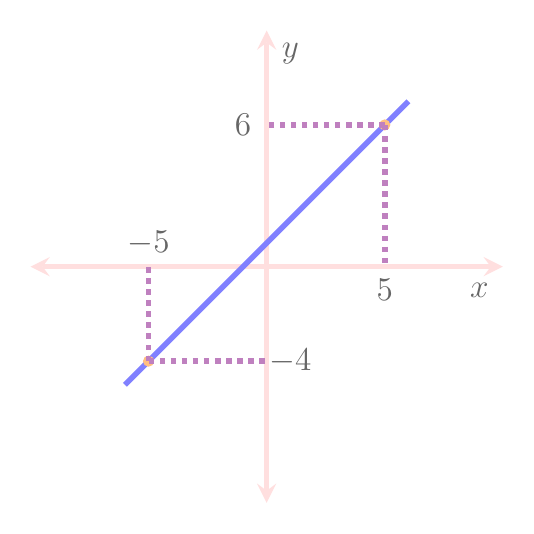
\begin{tikzpicture}[scale=0.3]
\tikzstyle{texto}=[draw=none,fill=none,black!60!white]
\tikzstyle{line}=[blue!50!white,line width=2pt]
\tikzstyle{line2}=[violet!50!white,line width=2pt]
\tikzstyle{eixo}=[pink!50!white,line width=2pt]

\tikzstyle{no}=[orange!50!white]

\draw[eixo,stealth-stealth] (-10,0) -- (10,0);
\draw[eixo,stealth-stealth] (0,-10) -- (0,10);
\draw[line] (-6,-5) -- (6,7);
\filldraw[no] (-5,-4) circle (6pt);
\filldraw[no] (5,6) circle (6pt);
\draw[dotted,line2] (-5,-4) -- (-5,0);
\draw[dotted,line2] (-5,-4) -- (0,-4);
\draw[dotted,line2] (5,6) -- (5,0);
\draw[dotted,line2] (5,6) -- (0,6);

\node[texto] at (9,-1) {\large$x$};
\node[texto] at (1,9) {\large$y$};
\node[texto] at (-5,1) {\large$-5$};
\node[texto] at (1,-4) {\large$-4$};
\node[texto] at (5,-1) {\large$5$};
\node[texto] at (-1,6) {\large$6$};

\end{tikzpicture}
\end{center}

$a=\dfrac{6-(-4)}{5-(-5)}=\dfrac{10}{10}=1$ \vspace{8px}

Deste modo, temos a seguinte função:

$y=1x+b$
\vspace{0.3cm}

Considerando o ponto $(6,5)$, temos:

$6=1 \cdot 5+b$

$6=5+b$

$b+5=6$

$b=6-5$

$b=1$

Após a definição de $b$ temos a função:

$f(x)=x+1$
\end{multicols}

\lfoot{\scriptsize © Copyright, Pratique Já}
\cfoot{\large \textcolor{bluebell}{pratiqueja.com}}
\end{document}